\graphicspath{{Figures/}}
\startchapter{Evaluation, Analysis and Comparisons}
\label{chapter:eval2}
In this chapter, we present a detailed comparison of our two approaches: Irregular neighborhood restructuring (ISFCA) and Confidence-based normative knowledge source (CSFCA) with other methods. We chose the standard social fabric algorithm by \citet{ali2016leveraged} and Tribe-PSO by \citet{chen2006tribe} for the purpose of comparison, as both of them utilize social structures and a tribal approach. 
\newline
We compare the approaches on each function with 10 and 30 dimensions. For each function, an overall comparison is presented regarding mean, median, best, and standard deviation (StdDev). Then, average fitness values of 10 experiments with different random generator settings are presented.
\section{Function 1: Bent Cigar Function}
In table \ref{tbl1_10} and figure \ref{func1_10}, we can see that both of our approaches (ISFCA and CSFCA) and TPSO outperform the standard SFCA impressively with 98\% and 55\% for optimization of 10 dimensions. In the case of 30-dimension optimization, ISFCA and CSFCA perform with 60\% and 42\% improvement respectively. 
\begin{table}[H]
	\caption{function-1, dimension-10}
	\begin{tabular}{|c|c|c|c|c|}
		\hline
		& \textbf{SFPSO} & \textbf{CSFEP} & \textbf{SFEP} & \textbf{TPSO} \\ \hline
		\textbf{Median} & 5.721885E+06 & 5.113078E+08 & 8.122664E+09 & 5.426664E+05 \\ \hline
		\textbf{Mean} & 1.576602E+08 & 4.091655E+09 & 9.246107E+09 & 2.479394E+08 \\ \hline
		\textbf{Best} & 5.711750E+06 & 9.279149E+05 & 9.908642E+08 & 5.415067E+05 \\ \hline
		\textbf{StdDev} & 3.066335E+08 & 6.639431E+09 & 8.500530E+09 & 3.993037E+08 \\ \hline
	\end{tabular}
	\label{tbl1_10}
\end{table}
\begin{figure}[H]
	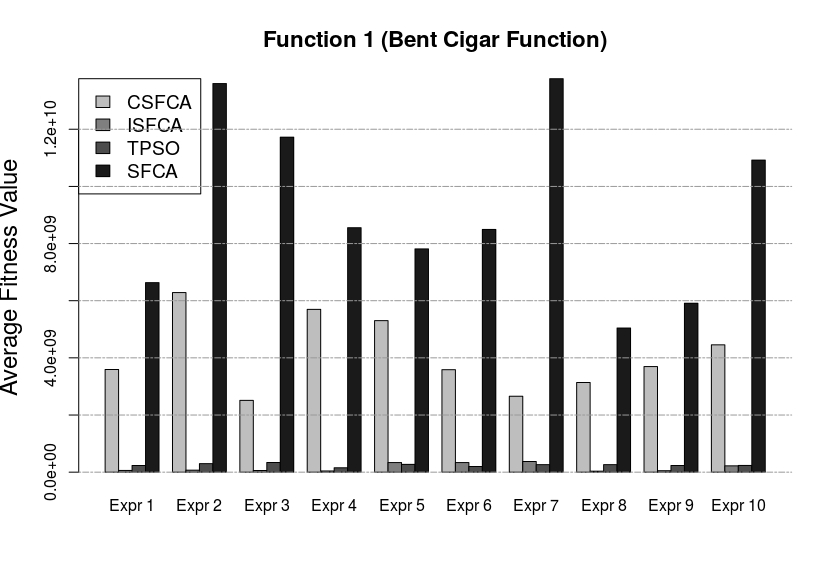
\includegraphics[scale=0.5]{func1_10}
	\centering
	\caption{Average fitness values for Function 1 with 10 dimensions}
	\label{func1_10}
\end{figure}
\begin{table}[H]
	\caption{function-1, dimension-30}
	\begin{tabular}{|c|c|c|c|c|}
		\hline
		& \textbf{SFPSO} & \textbf{CSFEP} & \textbf{SFEP} & \textbf{TPSO} \\ \hline
		\textbf{Median} & 1.224376E+10 & 9.035849E+09 & 3.381544E+10 & 1.223994E+10 \\ \hline
		\textbf{Mean} & 1.497176E+10 & 2.168689E+10 & 3.786293E+10 & 1.718683E+10 \\ \hline
		\textbf{Best} & 1.075684E+10 & 3.249525E+08 & 8.929425E+09 & 1.136511E+10 \\ \hline
		\textbf{StdDev} & 6.549615E+09 & 2.551255E+10 & 2.853221E+10 & 7.102879E+09 \\ \hline
	\end{tabular}
	\label{tbl1_30}
\end{table}
\begin{figure}[H]
	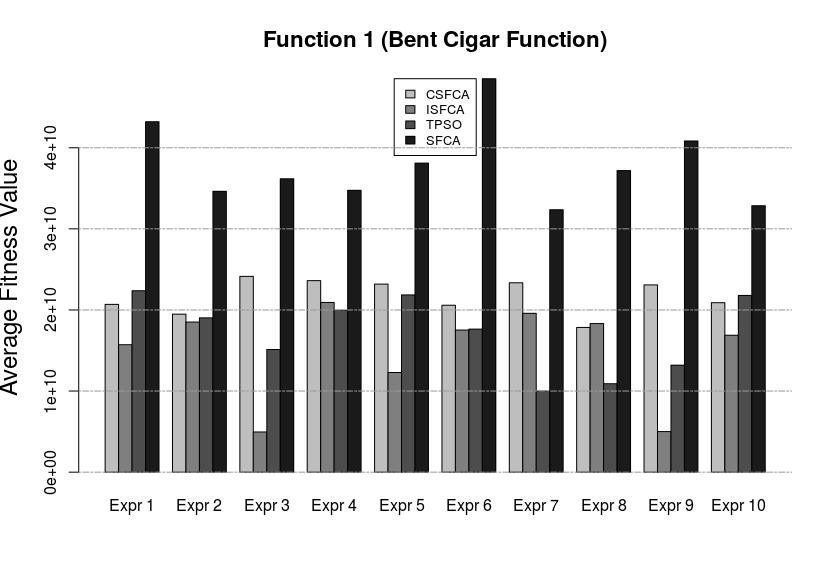
\includegraphics[scale=0.5]{func1_30}
	\centering
	\caption{Average fitness values for Function 1 with 30 dimensions}
	\label{func1_30}
\end{figure}

%\newpage

\section{Function 2: Discus Function}
As we can see in the table \ref{tbl2_10} and \ref{func2_10}, for 10-dimension optimization, ISFCA and CSFCA improve by 99\% and 42\% on the function 2. As explained in table \ref{tbl2_30} and \ref{func2_30}, they outperform the standard algorithm by 99\% and 95\% for 30-diemension optimization. 
\begin{table}[h]
	\caption{function-2, dimension-10}
	\begin{tabular}{|c|c|c|c|c|}
		\hline
		& \textbf{SFPSO} & \textbf{CSFEP} & \textbf{SFEP} & \textbf{TPSO} \\ \hline
		\textbf{Median} & 1.763602E+04 & 1.858882E+04 & 1.966669E+09 & 1.989622E+04 \\ \hline
		\textbf{Mean} & 1.970646E+04 & 2.045944E+09 & 3.574556E+09 & 2.202554E+04 \\ \hline
		\textbf{Best} & 1.690419E+04 & 1.426333E+04 & 2.467511E+04 & 1.722714E+04 \\ \hline
		\textbf{StdDev} & 5.285568E+03 & 4.083561E+09 & 4.508859E+09 & 5.505069E+03 \\ \hline
	\end{tabular}
	\label{tbl2_10}
\end{table}
\begin{figure}[h]
	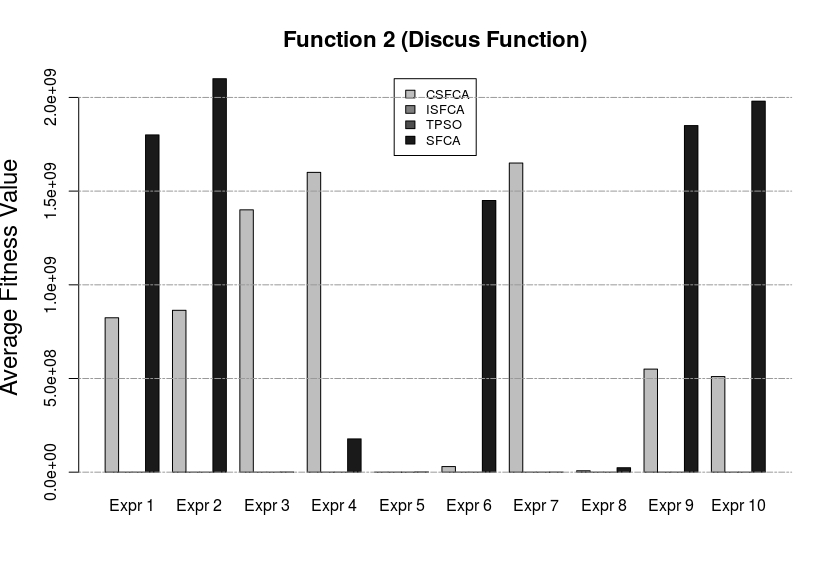
\includegraphics[scale=0.5]{func2_10}
	\centering
	\caption{Average fitness values for Function 2 with 10 dimensions}
	\label{func2_10}
\end{figure}
\begin{table}[h]
	\caption{function-2, dimension-30}
	\begin{tabular}{|c|c|c|c|c|}
		\hline
		& \textbf{SFPSO} & \textbf{CSFEP} & \textbf{SFEP} & \textbf{TPSO} \\ \hline
		\textbf{Median} & 7.057468E+04 & 6.106335E+04 & 8.669496E+07 & 1.338066E+05 \\ \hline
		\textbf{Mean} & 7.324758E+04 & 1.090201E+08 & 2.266584E+09 & 1.324195E+05 \\ \hline
		\textbf{Best} & 6.816396E+04 & 5.556673E+04 & 7.322705E+04 & 1.112664E+05 \\ \hline
		\textbf{StdDev} & 1.112414E+04 & 2.214664E+08 & 4.323029E+09 & 1.359207E+04 \\ \hline
	\end{tabular}
	\label{tbl2_30}
\end{table}
\begin{figure}[H]
	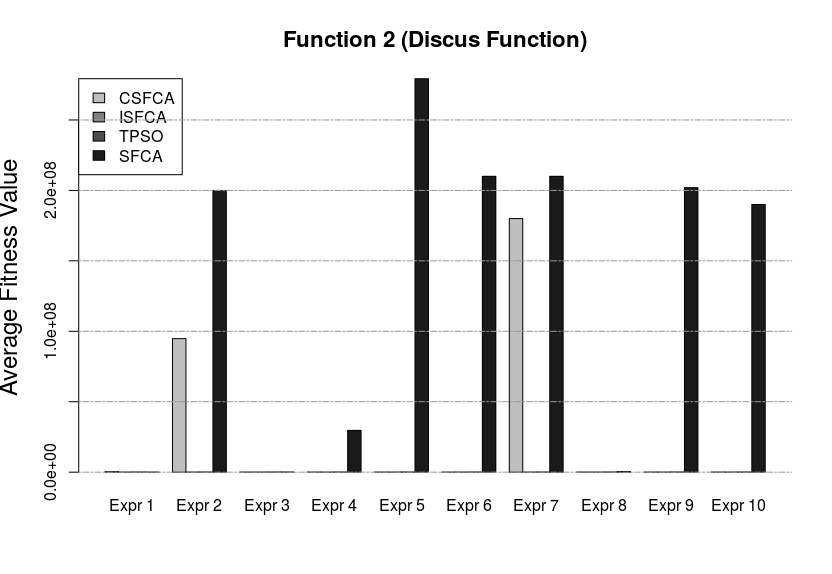
\includegraphics[scale=0.5]{func2_30}
	\centering
	\caption{Average fitness values for Function 2 with 30 dimensions}
	\label{func2_30}
\end{figure}

\section{Function 3: Weierstrass Function}
As you can see in Tables \ref{tbl3_10} and \ref{tbl3_30} and Figures \ref{func3_10} and \ref{func3_30}, the improvement of our approaches is trivial. However, it is still better than SFCA.
\begin{table}[h]
	\caption{function-3, dimension-10}
	\begin{tabular}{|c|c|c|c|c|}
		\hline
		& \textbf{SFPSO} & \textbf{CSFEP} & \textbf{SFEP} & \textbf{TPSO} \\ \hline
		\textbf{Median} & 3.053639E+02 & 3.088023E+02 & 3.106131E+02 & 3.059917E+02 \\ \hline
		\textbf{Mean} & 3.055362E+02 & 3.095236E+02 & 3.108567E+02 & 3.064904E+02 \\ \hline
		\textbf{Best} & 3.047026E+02 & 3.075572E+02 & 3.086619E+02 & 3.055813E+02 \\ \hline
		\textbf{StdDev} & 9.238688E-01 & 2.153735E+00 & 2.160320E+00 & 9.113892E-01 \\ \hline
	\end{tabular}
	\label{tbl3_10}
\end{table}

\begin{figure}[h]
	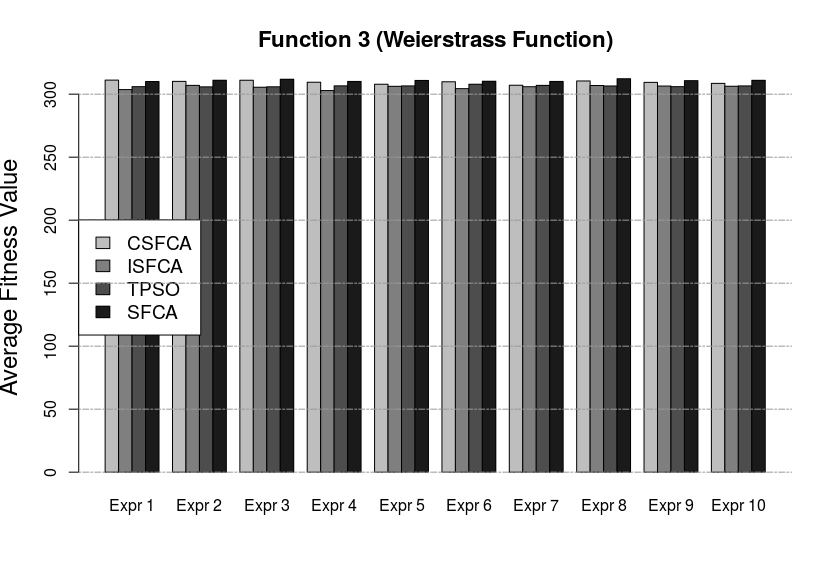
\includegraphics[scale=0.5]{func3_10}
	\centering
	\caption{Average fitness values for Function 3 with 10 dimensions}
	\label{func3_10}
\end{figure}

\begin{table}[h]
	\caption{function-3, dimension-30}
	\begin{tabular}{|c|c|c|c|c|}
		\hline
		& \textbf{SFPSO} & \textbf{CSFEP} & \textbf{SFEP} & \textbf{TPSO} \\ \hline
		\textbf{Median} & 3.288747E+02 & 3.395129E+02 & 3.414242E+02 & 3.276385E+02 \\ \hline
		\textbf{Mean} & 3.307785E+02 & 3.400480E+02 & 3.410312E+02 & 3.305742E+02 \\ \hline
		\textbf{Best} & 3.274619E+02 & 3.352212E+02 & 3.360418E+02 & 3.275333E+02 \\ \hline
		\textbf{StdDev} & 3.242337E+00 & 4.748334E+00 & 4.694844E+00 & 3.905358E+00 \\ \hline
	\end{tabular}
	\label{tbl3_30}
\end{table}
\begin{figure}[H]
	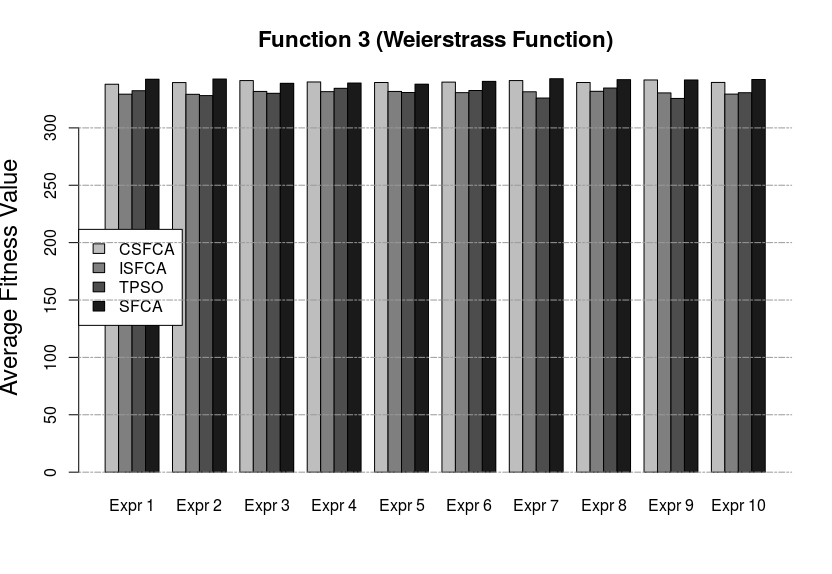
\includegraphics[scale=0.5]{func3_30}
	\centering
	\caption{Average fitness values for Function 3 with 30 dimensions}
	\label{func3_30}
\end{figure}

\section{Function 4: Modified Schwefel's Function}
Table \ref{tbl4_10} and figure \ref{func4_10} show that in the case 10-dimension optimizatoin, ISFCA performs better by 18\% and CSFCA by 19\%. However, for the 30-dimension case, only CSFCA outperform SFCA by 21\% as shown in Table \ref{tbl4_30} and Figure \ref{func4_30}.
\begin{table}[h]
	\caption{function-4, dimension-10}
	\begin{tabular}{|c|c|c|c|c|}
		\hline
		& \textbf{SFPSO} & \textbf{CSFEP} & \textbf{SFEP} & \textbf{TPSO} \\ \hline
		\textbf{Median} & 1.374025E+03 & 1.198259E+03 & 1.740208E+03 & 1.326440E+03 \\ \hline
		\textbf{Mean} & 1.401458E+03 & 1.392015E+03 & 1.725446E+03 & 1.391022E+03 \\ \hline
		\textbf{Best} & 1.249122E+03 & 6.135802E+02 & 8.405862E+02 & 1.201363E+03 \\ \hline
		\textbf{StdDev} & 1.709634E+02 & 8.047924E+02 & 8.388958E+02 & 2.174364E+02 \\ \hline
	\end{tabular}
	\label{tbl4_10}
\end{table}

\begin{figure}[h]
	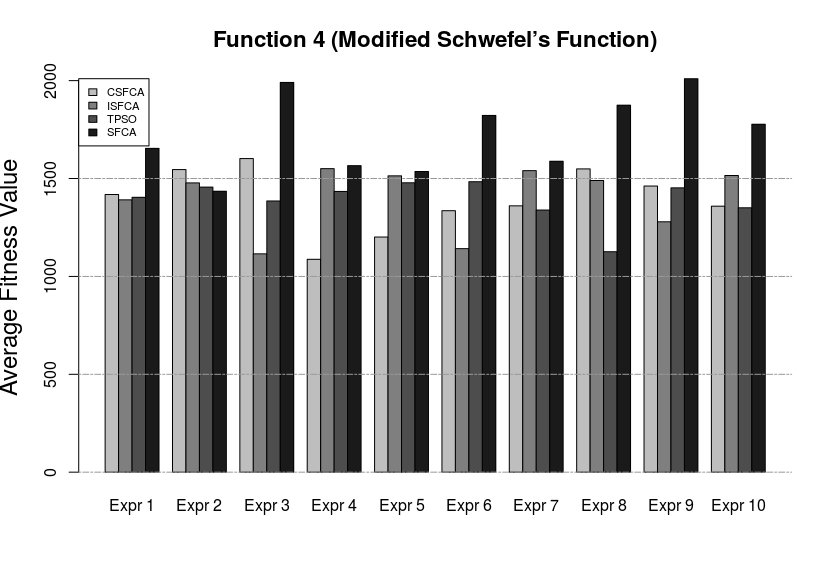
\includegraphics[scale=0.5]{func4_10}
	\centering
	\caption{Average fitness values for Function 4 with 10 dimensions}
	\label{func4_10}
\end{figure}

\begin{table}[h]
	\caption{function-4, dimension-30}
	\begin{tabular}{|c|c|c|c|c|}
		\hline
		& \textbf{SFPSO} & \textbf{CSFEP} & \textbf{SFEP} & \textbf{TPSO} \\ \hline
		\textbf{Median} & 6.870764E+03 & 5.098037E+03 & 6.819341E+03 & 7.117825E+03 \\ \hline
		\textbf{Mean} & 6.964474E+03 & 4.998230E+03 & 6.375121E+03 & 7.270199E+03 \\ \hline
		\textbf{Best} & 6.625647E+03 & 1.377132E+03 & 3.463489E+03 & 6.882440E+03 \\ \hline
		\textbf{StdDev} & 4.205720E+02 & 3.054933E+03 & 2.436783E+03 & 4.387157E+02 \\ \hline
	\end{tabular}
	\label{tbl4_30}
\end{table}

\begin{figure}[H]
	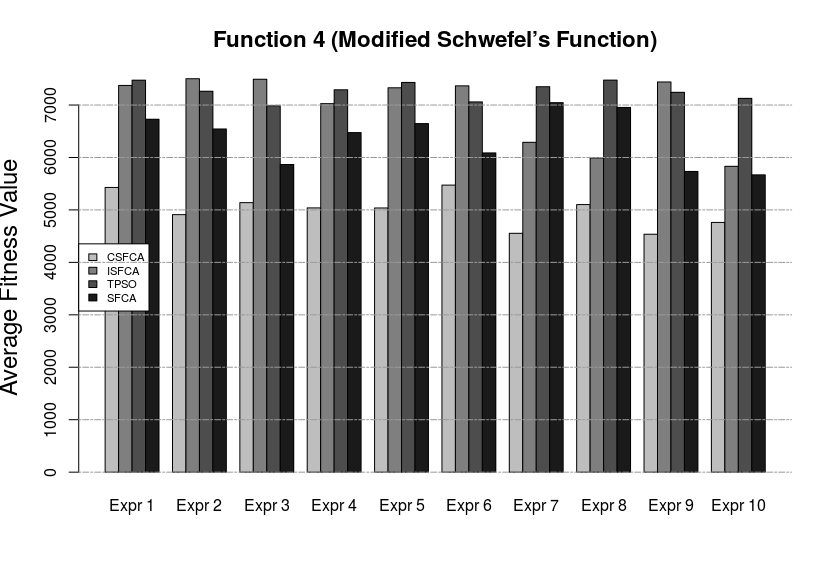
\includegraphics[scale=0.5]{func4_30}
	\centering
	\caption{Average fitness values for Function 4 with 30 dimensions}
	\label{func4_30}
\end{figure}

\section{Function 5: Katsuura Function}
As you can in Tables \ref{tbl5_10} and \ref{tbl5_30} and Figures \ref{func5_10} and \ref{func5_30}, the results of all the approaches are almost the same.
\begin{table}[h]
	\caption{function-5, dimension-10}
	\begin{tabular}{|c|c|c|c|c|}
		\hline
		& \textbf{SFPSO} & \textbf{CSFEP} & \textbf{SFEP} & \textbf{TPSO} \\ \hline
		\textbf{Median} & 5.012550E+02 & 5.014254E+02 & 5.019767E+02 & 5.012505E+02 \\ \hline
		\textbf{Mean} & 5.013300E+02 & 5.017117E+02 & 5.023857E+02 & 5.013223E+02 \\ \hline
		\textbf{Best} & 5.010726E+02 & 5.007002E+02 & 5.011836E+02 & 5.011289E+02 \\ \hline
		\textbf{StdDev} & 2.684750E-01 & 1.132619E+00 & 1.339239E+00 & 2.057213E-01 \\ \hline
	\end{tabular}
	\label{tbl5_10}
\end{table}

\begin{figure}[h]
	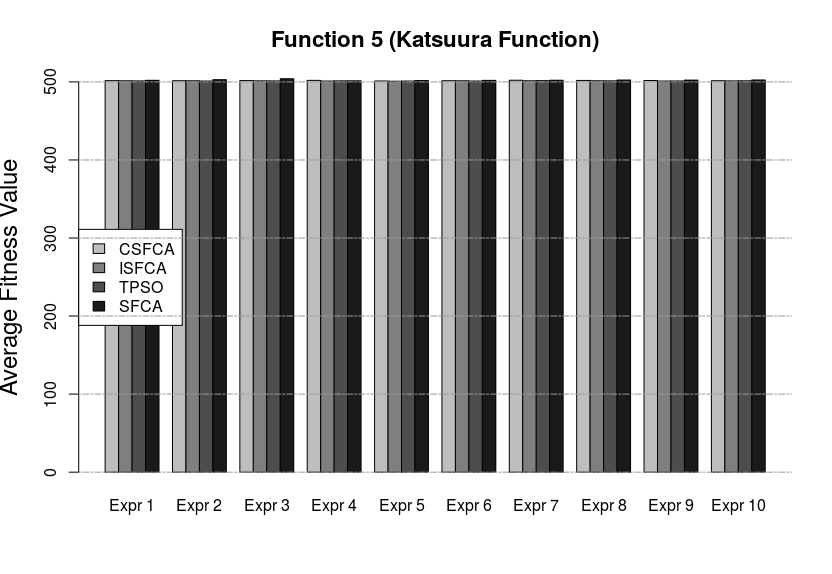
\includegraphics[scale=0.5]{func5_10}
	\centering
	\caption{Average fitness values for Function 5 with 10 dimensions}
	\label{func5_10}
\end{figure}

\begin{table}[h]
	\caption{function-5, dimension-30}
	\begin{tabular}{|c|c|c|c|c|}
		\hline
		& \textbf{SFPSO} & \textbf{CSFEP} & \textbf{SFEP} & \textbf{TPSO} \\ \hline
		\textbf{Median} & 5.029073E+02 & 5.025217E+02 & 5.030453E+02 & 5.028359E+02 \\ \hline
		\textbf{Mean} & 5.030805E+02 & 5.031380E+02 & 5.036162E+02 & 5.029678E+02 \\ \hline
		\textbf{Best} & 5.028153E+02 & 5.016618E+02 & 5.020560E+02 & 5.026209E+02 \\ \hline
		\textbf{StdDev} & 3.548877E-01 & 1.669277E+00 & 1.678840E+00 & 3.015601E-01 \\ \hline
	\end{tabular}
	\label{tbl5_30}
\end{table}
\begin{figure}[H]
	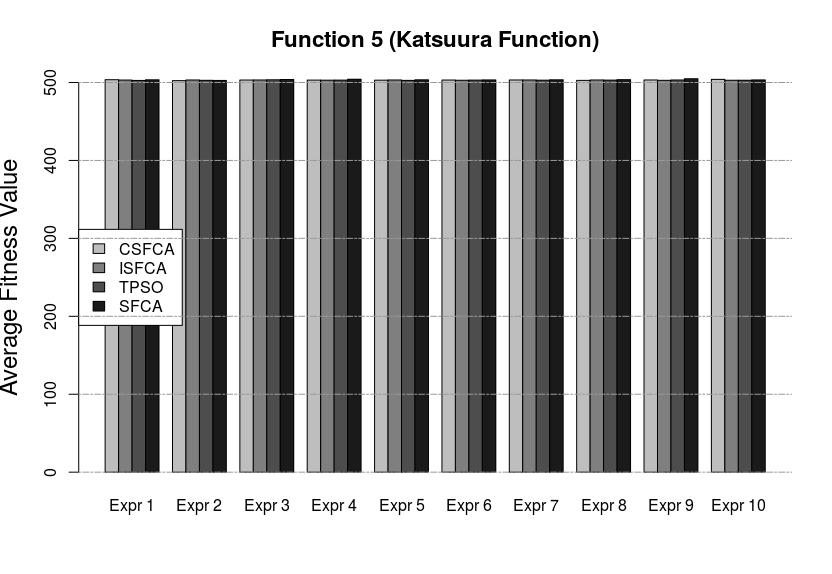
\includegraphics[scale=0.5]{func5_30}
	\centering
	\caption{Average fitness values for Function 5 with 30 dimensions}
	\label{func5_30}
\end{figure}

\newpage

\section{Function 6: HappyCat Function}
As you can see in Tables \ref{tbl6_10} and \ref{tbl6_30} and Figures \ref{func6_10} and \ref{func6_10}, the improvement of our approaches is trivial.
\begin{table}[h]
	\caption{function-6, dimension-10}
	\begin{tabular}{|c|c|c|c|c|}
		\hline
		& \textbf{SFPSO} & \textbf{CSFEP} & \textbf{SFEP} & \textbf{TPSO} \\ \hline
		\textbf{Median} & 6.004688E+02 & 6.015392E+02 & 6.033087E+02 & 6.005062E+02 \\ \hline
		\textbf{Mean} & 6.005623E+02 & 6.025225E+02 & 6.036813E+02 & 6.009515E+02 \\ \hline
		\textbf{Best} & 6.004334E+02 & 6.005685E+02 & 6.018524E+02 & 6.005062E+02 \\ \hline
		\textbf{StdDev} & 3.200289E-01 & 2.304279E+00 & 1.898523E+00 & 6.229300E-01 \\ \hline
	\end{tabular}
	\label{tbl6_10}
\end{table}

\begin{figure}[h]
	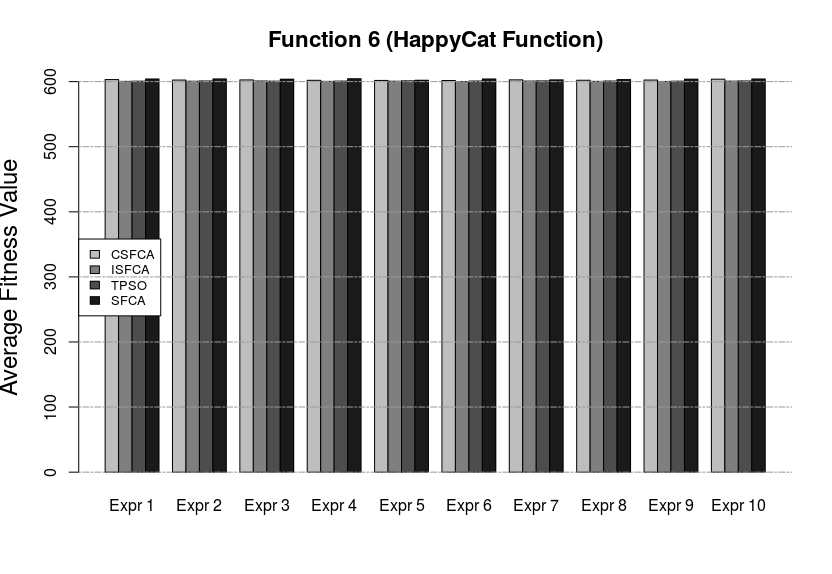
\includegraphics[scale=0.5]{func6_10}
	\centering
	\caption{Average fitness values for Function 6 with 10 dimensions}
	\label{func6_10}
\end{figure}

\begin{table}[h]
	\caption{function-6, dimension-30}
	\begin{tabular}{|c|c|c|c|c|}
		\hline
		& \textbf{SFPSO} & \textbf{CSFEP} & \textbf{SFEP} & \textbf{TPSO} \\ \hline
		\textbf{Median} & 6.025572E+02 & 6.038615E+02 & 6.054925E+02 & 6.010077E+02 \\ \hline
		\textbf{Mean} & 6.030236E+02 & 6.039768E+02 & 6.056628E+02 & 6.019309E+02 \\ \hline
		\textbf{Best} & 6.024192E+02 & 6.010681E+02 & 6.041570E+02 & 6.010077E+02 \\ \hline
		\textbf{StdDev} & 7.579661E-01 & 2.740738E+00 & 1.433152E+00 & 1.224478E+00 \\ \hline
	\end{tabular}
	\label{tbl6_30}
\end{table}
\begin{figure}[H]
	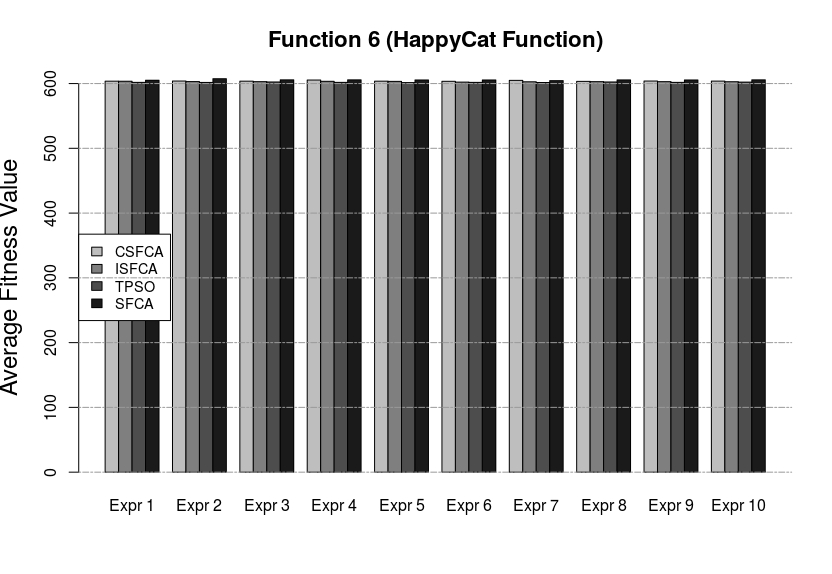
\includegraphics[scale=0.5]{func6_30}
	\centering
	\caption{Average fitness values for Function 6 with 30 dimensions}
	\label{func6_30}
\end{figure}

\newpage

\section{Function 7: HGBat Function}
As you can see in Tables \ref{tbl7_10} and \ref{tbl7_30} and Figures \ref{func7_10} and \ref{func7_10}, the improvement of our approaches is not so much. In the case of 10-dimension optimization, it is about 5\% and for the 30-dimension case, it is about 9\%. 
\begin{table}[h]
	\caption{function-7, dimension-10}
	\begin{tabular}{|c|c|c|c|c|}
		\hline
		& \textbf{SFPSO} & \textbf{CSFEP} & \textbf{SFEP} & \textbf{TPSO} \\ \hline
		\textbf{Median} & 7.008041E+02 & 7.081532E+02 & 7.341129E+02 & 7.004902E+02 \\ \hline
		\textbf{Mean} & 7.019942E+02 & 7.260979E+02 & 7.418000E+02 & 7.038384E+02 \\ \hline
		\textbf{Best} & 7.006188E+02 & 7.007965E+02 & 7.100632E+02 & 7.004902E+02 \\ \hline
		\textbf{StdDev} & 2.635216E+00 & 3.539268E+01 & 3.490056E+01 & 5.486938E+00 \\ \hline
	\end{tabular}
	\label{tbl7_10}
\end{table}

\begin{figure}[h]
	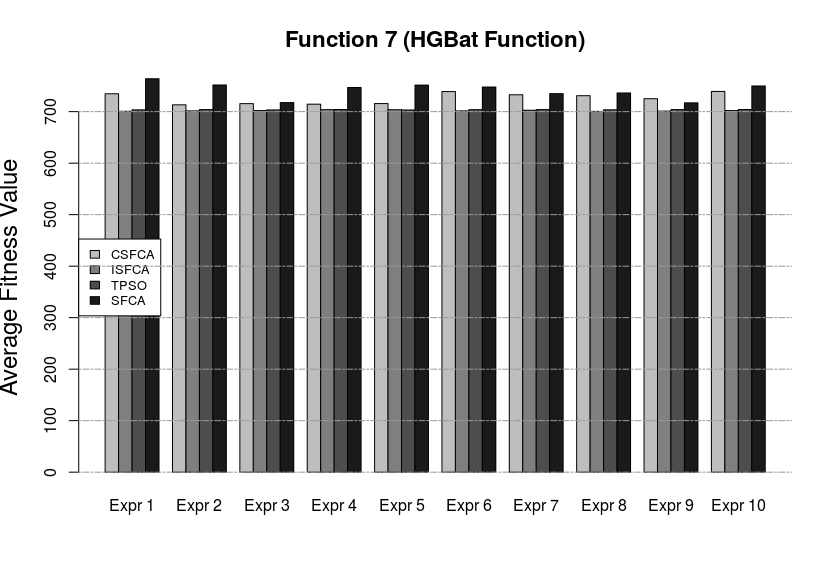
\includegraphics[scale=0.5]{func7_10}
	\centering
	\caption{Average fitness values for Function 7 with 10 dimensions}
	\label{func7_10}
\end{figure}

\begin{table}[h]
	\caption{function-7, dimension-30}
	\begin{tabular}{|c|c|c|c|c|}
		\hline
		& \textbf{SFPSO} & \textbf{CSFEP} & \textbf{SFEP} & \textbf{TPSO} \\ \hline
		\textbf{Median} & 7.291294E+02 & 7.477774E+02 & 8.042494E+02 & 7.280204E+02 \\ \hline
		\textbf{Mean} & 7.389013E+02 & 7.605963E+02 & 8.116680E+02 & 7.498652E+02 \\ \hline
		\textbf{Best} & 7.271223E+02 & 7.024000E+02 & 7.544377E+02 & 7.262179E+02 \\ \hline
		\textbf{StdDev} & 1.569694E+01 & 5.981939E+01 & 5.740507E+01 & 2.791729E+01 \\ \hline
	\end{tabular}
	\label{tbl7_30}
\end{table}
\begin{figure}[H]
	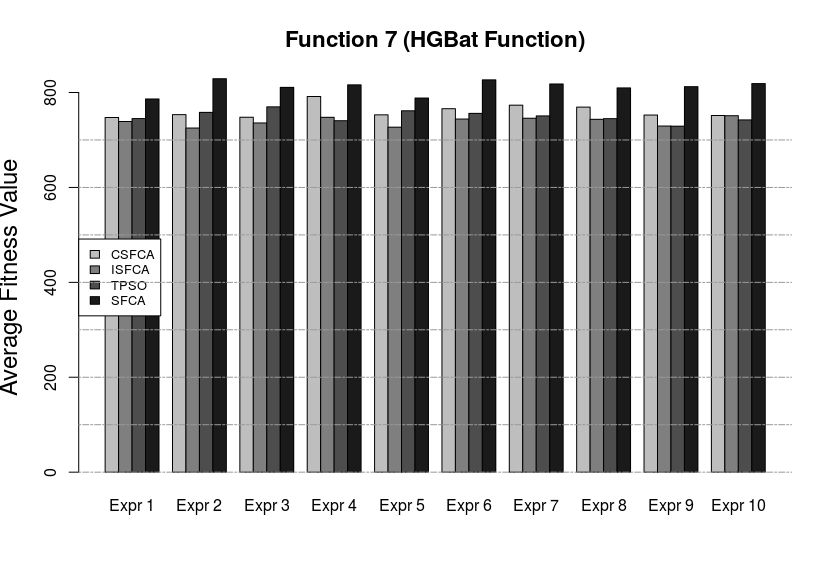
\includegraphics[scale=0.5]{func7_30}
	\centering
	\caption{Average fitness values for Function 7 with 30 dimensions}
	\label{func7_30}
\end{figure}

\section{Function 8: Griewank's plus Rosenbrock's Function}
In table \ref{tbl8_10} and figure \ref{func8_10}, we can see that both of our approaches (ISFCA and CSFCA) and TPSO outperform the standard SFCA impressively with 99\% and 77\% for optimization of 10 dimensions. In the case of 30-dimension optimization, ISFCA and CSFCA perform with 97\% and 52\% improvement respectively as shown in Table \ref{tbl8_30} and Figure \ref{func8_30}. 
\begin{table}[h]
	\caption{function-8, dimension-10}
	\begin{tabular}{|c|c|c|c|c|}
		\hline
		& \textbf{SFPSO} & \textbf{CSFEP} & \textbf{SFEP} & \textbf{TPSO} \\ \hline
		\textbf{Median} & 8.060488E+02 & 4.762535E+03 & 5.638811E+05 & 8.057399E+02 \\ \hline
		\textbf{Mean} & 8.327824E+02 & 3.080861E+05 & 1.374142E+06 & 8.319941E+02 \\ \hline
		\textbf{Best} & 8.060488E+02 & 8.475602E+02 & 4.118304E+03 & 8.057399E+02 \\ \hline
		\textbf{StdDev} & 1.428379E+02 & 5.970746E+05 & 1.940514E+06 & 7.254239E+01 \\ \hline
	\end{tabular}
	\label{tbl8_10}
\end{table}

\begin{figure}[h]
	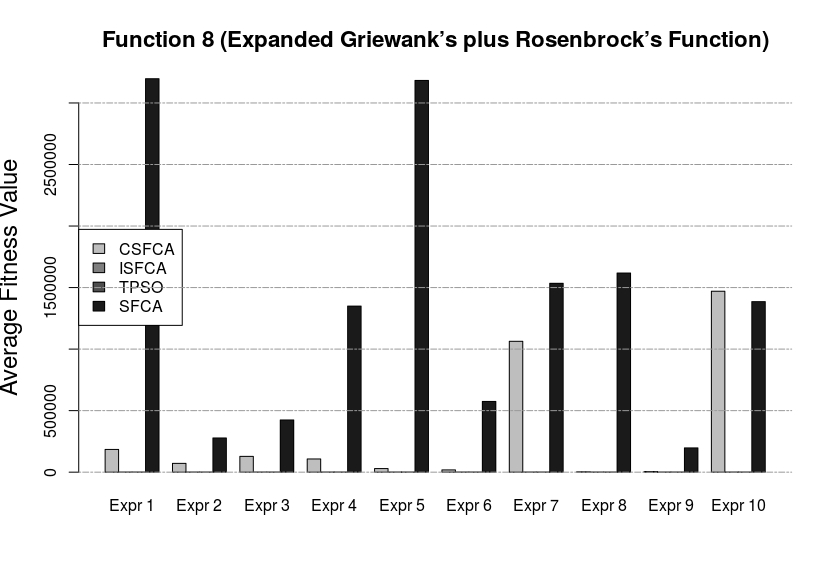
\includegraphics[scale=0.5]{func8_10}
	\centering
	\caption{Average fitness values for Function 8 with 10 dimensions}
	\label{func8_10}
\end{figure}

\begin{table}[h]
	\caption{function-8, dimension-30}
	\begin{tabular}{|c|c|c|c|c|}
		\hline
		& \textbf{SFPSO} & \textbf{CSFEP} & \textbf{SFEP} & \textbf{TPSO} \\ \hline
		\textbf{Median} & 1.139271E+05 & 3.872060E+05 & 3.562129E+06 & 8.406430E+05 \\ \hline
		\textbf{Mean} & 3.363145E+05 & 7.477703E+06 & 1.541796E+07 & 1.645666E+06 \\ \hline
		\textbf{Best} & 5.240269E+04 & 1.095824E+03 & 8.508643E+04 & 4.126489E+05 \\ \hline
		\textbf{StdDev} & 6.891847E+05 & 1.270040E+07 & 2.340250E+07 & 1.667678E+06 \\ \hline
	\end{tabular}
	\label{tbl8_30}
\end{table}
\begin{figure}[H]
	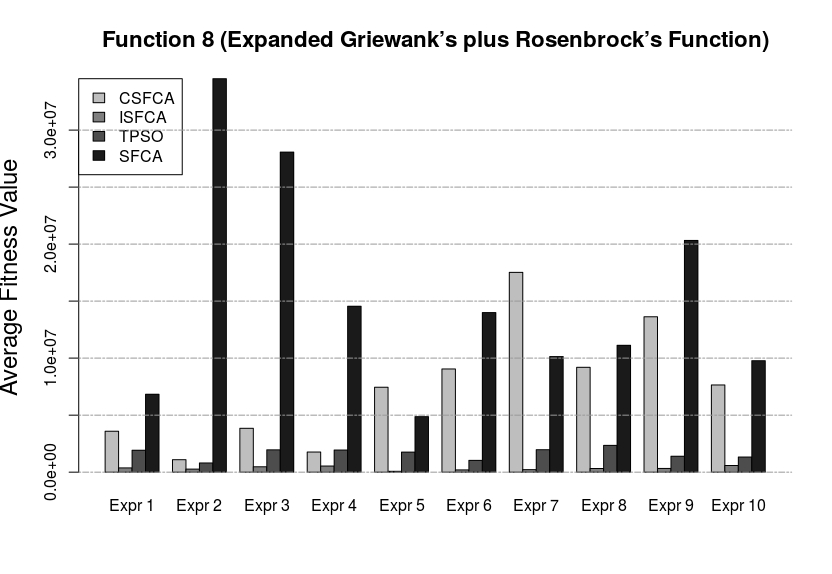
\includegraphics[scale=0.5]{func8_30}
	\centering
	\caption{Average fitness values for Function 8 with 30 dimensions}
	\label{func8_30}
\end{figure}

\section{Function 9: Expanded Scaffer's F6 Function}
In Tables \ref{tbl9_10} and \ref{tbl9_30} and Figures \ref{func9_10} and \ref{func9_30}, we can see that there is not a considerable improvement and all the methods perform almost the same.
\begin{table}[h]
	\caption{function-9, dimension-10}
	\begin{tabular}{|c|c|c|c|c|}
		\hline
		& \textbf{SFPSO} & \textbf{CSFEP} & \textbf{SFEP} & \textbf{TPSO} \\ \hline
		\textbf{Median} & 9.036094E+02 & 9.035775E+02 & 9.037811E+02 & 9.035661E+02 \\ \hline
		\textbf{Mean} & 9.036469E+02 & 9.036343E+02 & 9.038043E+02 & 9.036178E+02 \\ \hline
		\textbf{Best} & 9.035325E+02 & 9.032589E+02 & 9.033602E+02 & 9.035094E+02 \\ \hline
		\textbf{StdDev} & 1.008688E-01 & 3.372815E-01 & 4.187602E-01 & 1.037992E-01 \\ \hline
	\end{tabular}
	\label{tbl9_10}
\end{table}

\begin{figure}[h]
	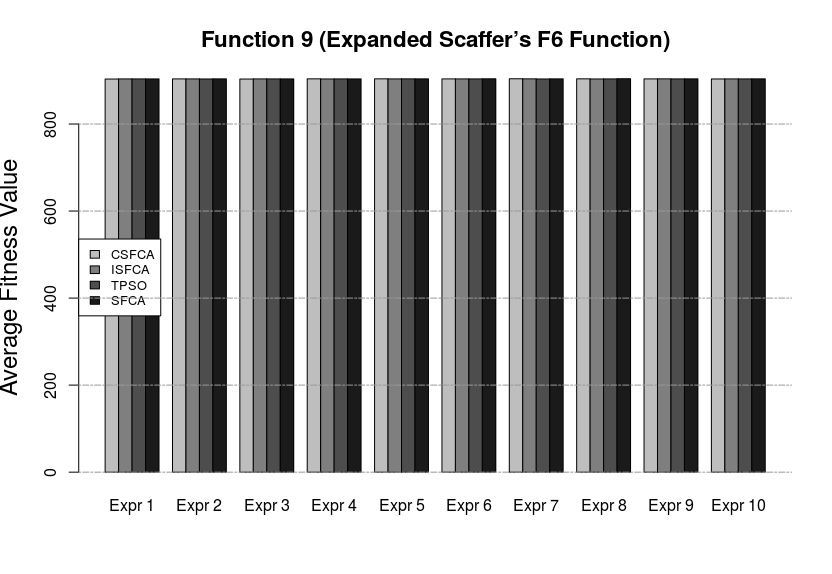
\includegraphics[scale=0.5]{func9_10}
	\centering
	\caption{Average fitness values for Function 9 with 10 dimensions}
	\label{func9_10}
\end{figure}

\begin{table}[h]
	\caption{function-9, dimension-30}
	\begin{tabular}{|c|c|c|c|c|}
		\hline
		& \textbf{SFPSO} & \textbf{CSFEP} & \textbf{SFEP} & \textbf{TPSO} \\ \hline
		\textbf{Median} & 9.134898E+02 & 9.134569E+02 & 9.136834E+02 & 9.135212E+02 \\ \hline
		\textbf{Mean} & 9.135258E+02 & 9.133575E+02 & 9.136351E+02 & 9.135977E+02 \\ \hline
		\textbf{Best} & 9.133757E+02 & 9.126562E+02 & 9.131192E+02 & 9.134243E+02 \\ \hline
		\textbf{StdDev} & 1.312660E-01 & 5.882330E-01 & 4.913793E-01 & 1.390313E-01 \\ \hline
	\end{tabular}
	\label{tbl9_30}
\end{table}
\begin{figure}[H]
	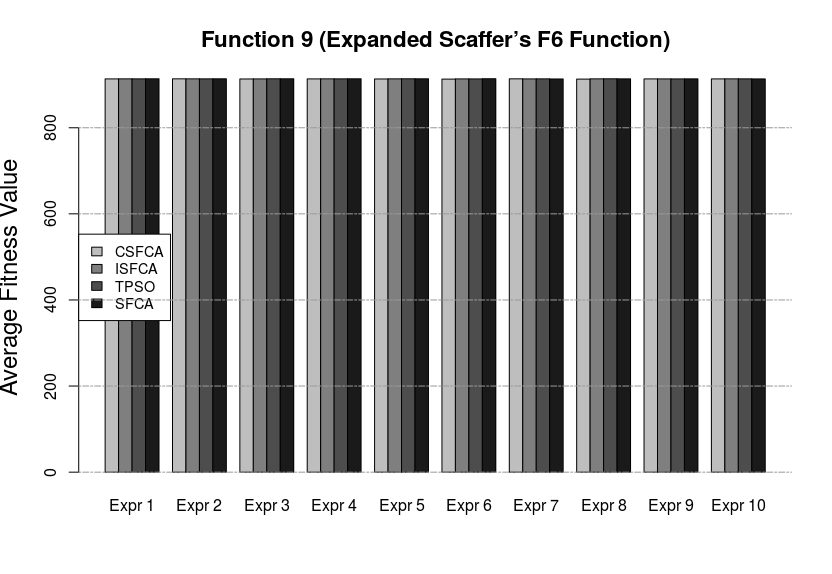
\includegraphics[scale=0.5]{func9_30}
	\centering
	\caption{Average fitness values for Function 9 with 30 dimensions}
	\label{func9_30}
\end{figure}

\section{Function 10: Hybrid Function 1}
In the 10-dimension case, Table \ref{tbl10_10} and Figure \ref{func10_10} show an impressive improvement for both ISFCA and CSFCA approaches by 99\% and 77\% respectively. For the 30-dimension case, ISFCA and CSFCA outperform SFCA by 97\% and 51\% respectively as shown in Table \ref{tbl10_30} and Figure \ref{func10_30}.
\begin{table}[h]
	\caption{function-10, dimension-10}
	\begin{tabular}{|c|c|c|c|c|}
		\hline
		& \textbf{SFPSO} & \textbf{CSFEP} & \textbf{SFEP} & \textbf{TPSO} \\ \hline
		\textbf{Median} & 5.078678E+04 & 5.565684E+05 & 1.462417E+06 & 3.479607E+04 \\ \hline
		\textbf{Mean} & 6.855882E+04 & 1.390710E+06 & 1.250589E+07 & 6.576307E+04 \\ \hline
		\textbf{Best} & 2.148022E+04 & 2.365329E+03 & 6.578523E+03 & 1.417589E+04 \\ \hline
		\textbf{StdDev} & 7.234730E+04 & 1.778552E+06 & 2.276703E+07 & 7.783437E+04 \\ \hline
	\end{tabular}
	\label{tbl10_10}
\end{table}

\begin{figure}[h]
	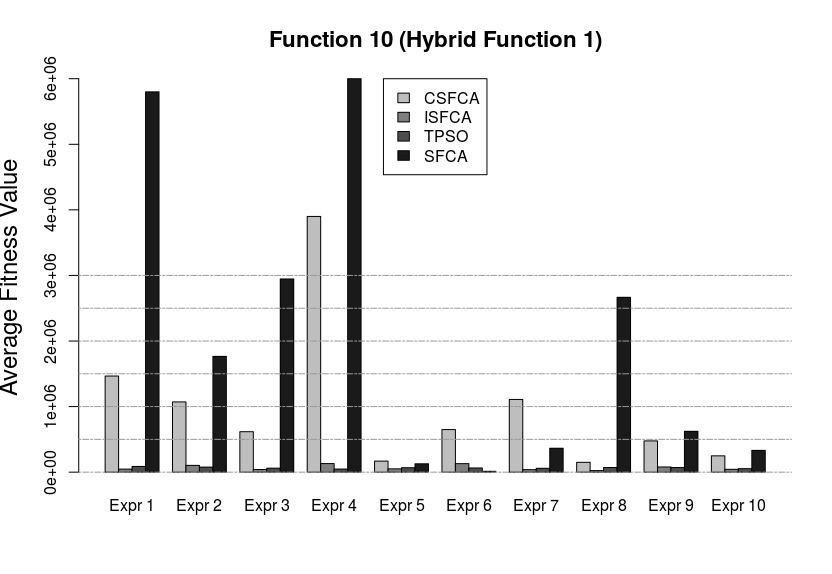
\includegraphics[scale=0.5]{func10_10}
	\centering
	\caption{Average fitness values for Function 10 with 10 dimensions}
	\label{func10_10}
\end{figure}

\begin{table}[h]
	\caption{function-10, dimension-30}
	\begin{tabular}{|c|c|c|c|c|}
		\hline
		& \textbf{SFPSO} & \textbf{CSFEP} & \textbf{SFEP} & \textbf{TPSO} \\ \hline
		\textbf{Median} & 1.257686E+07 & 2.886032E+07 & 7.068932E+07 & 1.524856E+07 \\ \hline
		\textbf{Mean} & 1.288355E+07 & 5.268560E+07 & 7.171894E+07 & 1.914266E+07 \\ \hline
		\textbf{Best} & 6.072906E+06 & 2.225892E+06 & 8.682100E+06 & 1.311979E+07 \\ \hline
		\textbf{StdDev} & 7.703664E+06 & 5.803312E+07 & 5.952516E+07 & 8.464172E+06 \\ \hline
	\end{tabular}
	\label{tbl10_30}
\end{table}
\begin{figure}[H]
	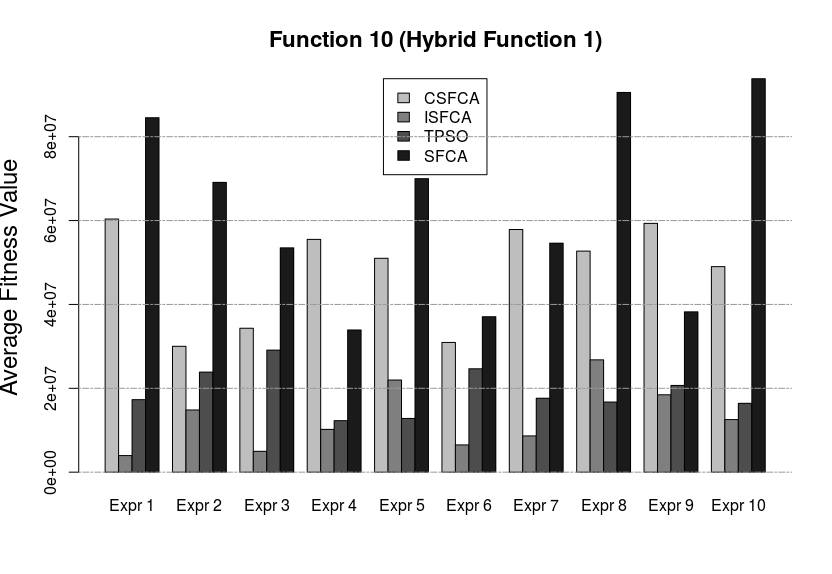
\includegraphics[scale=0.5]{func10_30}
	\centering
	\caption{Average fitness values for Function 10 with 30 dimensions}
	\label{func10_30}
\end{figure}

\section{Function 11: Hybrid Function 2}
 Table \ref{tbl11_10} and Figure \ref{func11_10} show a trivial improvement for the 10-dimension case. On the other hand, Table \ref{tbl11_30} and Figure \ref{func11_30} explain that ISFCA and CSFCA outperform the standard algorithm by 30\% and 15\% respectively.
\begin{table}[h]
	\caption{function-11, dimension-10}
	\begin{tabular}{|c|c|c|c|c|}
		\hline
		& \textbf{SFPSO} & \textbf{CSFEP} & \textbf{SFEP} & \textbf{TPSO} \\ \hline
		\textbf{Median} & 1.104725E+03 & 1.109982E+03 & 1.111399E+03 & 1.104917E+03 \\ \hline
		\textbf{Mean} & 1.105085E+03 & 1.137076E+03 & 1.140188E+03 & 1.105442E+03 \\ \hline
		\textbf{Best} & 1.104062E+03 & 1.106581E+03 & 1.105492E+03 & 1.104723E+03 \\ \hline
		\textbf{StdDev} & 1.339530E+00 & 5.229237E+01 & 4.994351E+01 & 9.340507E-01 \\ \hline
	\end{tabular}
	\label{tbl11_10}
\end{table}

\begin{figure}[h]
	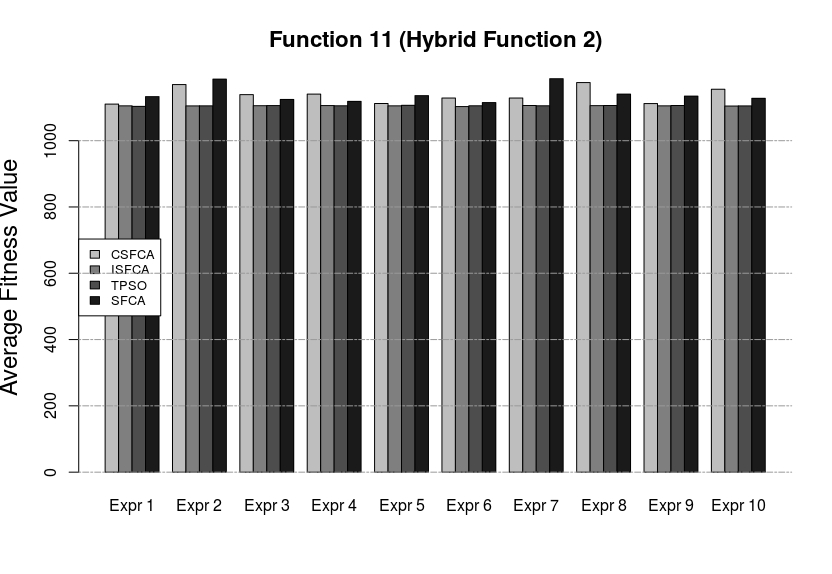
\includegraphics[scale=0.5]{func11_10}
	\centering
	\caption{Average fitness values for Function 11 with 10 dimensions}
	\label{func11_10}
\end{figure}

\begin{table}[h]
	\caption{function-11, dimension-30}
	\begin{tabular}{|c|c|c|c|c|}
		\hline
		& \textbf{SFPSO} & \textbf{CSFEP} & \textbf{SFEP} & \textbf{TPSO} \\ \hline
		\textbf{Median} & 1.188478E+03 & 1.246676E+03 & 1.561269E+03 & 1.134562E+03 \\ \hline
		\textbf{Mean} & 1.197912E+03 & 1.456495E+03 & 1.724513E+03 & 1.174516E+03 \\ \hline
		\textbf{Best} & 1.153360E+03 & 1.155965E+03 & 1.290852E+03 & 1.134562E+03 \\ \hline
		\textbf{StdDev} & 4.334944E+01 & 4.589486E+02 & 5.277303E+02 & 6.235017E+01 \\ \hline
	\end{tabular}
	\label{tbl11_30}
\end{table}
\begin{figure}[H]
	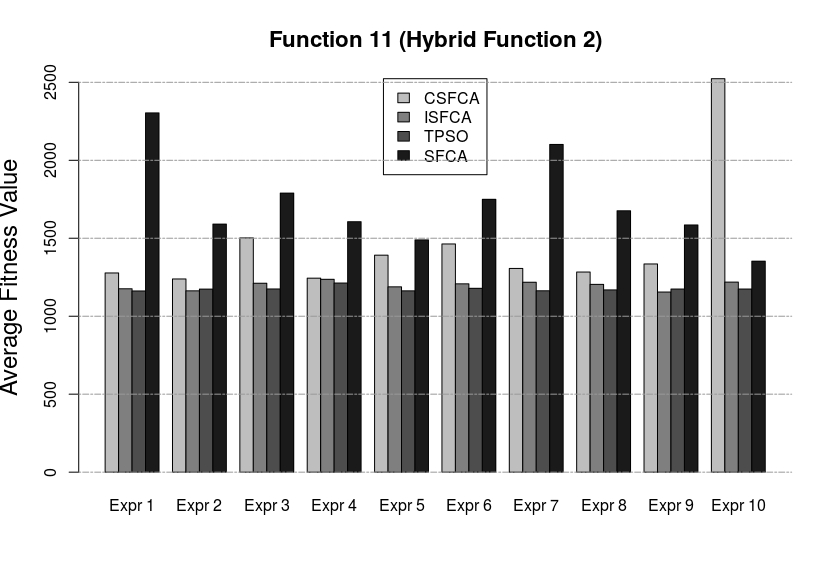
\includegraphics[scale=0.5]{func11_30}
	\centering
	\caption{Average fitness values for Function 11 with 30 dimensions}
	\label{func11_30}
\end{figure}

\section{Function 12: Hybrid Function 3}
Both of ISFCA and CSFCA approaches perform much better than the standard algorithm in both 10-dimension and 30-dimension scenarios. Table \ref{tbl12_10} and Figure \ref{func12_10} show that ISFCA and CSFCA improve the performance by 93\% and 82\% for the 10-dimension case. Table \ref{tbl12_30} and Figure \ref{func12_30} indicate that ISFCA and CSFCA improve the peformance by 99\% and 68\% for the 30-dimension case.
\begin{table}[h]
	\caption{function-12, dimension-10}
	\begin{tabular}{|c|c|c|c|c|}
		\hline
		& \textbf{SFPSO} & \textbf{CSFEP} & \textbf{SFEP} & \textbf{TPSO} \\ \hline
		\textbf{Median} & 1.278429E+03 & 1.470304E+03 & 2.561160E+03 & 1.274117E+03 \\ \hline
		\textbf{Mean} & 1.284340E+03 & 3.740383E+03 & 2.109208E+04 & 1.290392E+03 \\ \hline
		\textbf{Best} & 1.247398E+03 & 1.342194E+03 & 1.419410E+03 & 1.259420E+03 \\ \hline
		\textbf{StdDev} & 4.080435E+01 & 4.569942E+03 & 3.705284E+04 & 4.016558E+01 \\ \hline
	\end{tabular}
	\label{tbl12_10}
\end{table}

\begin{figure}[h]
	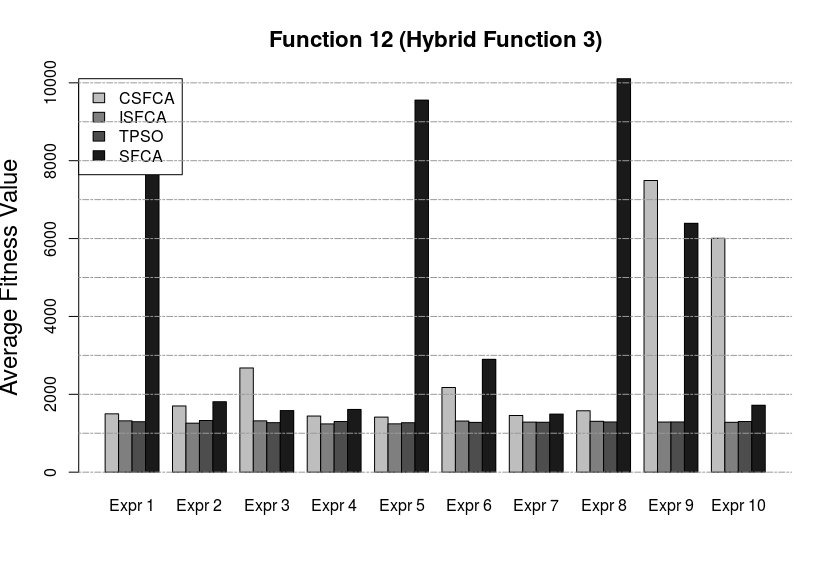
\includegraphics[scale=0.5]{func12_10}
	\centering
	\caption{Average fitness values for Function 12 with 10 dimensions}
	\label{func12_10}
\end{figure}

\begin{table}[h]
	\caption{function-12, dimension-30}
	\begin{tabular}{|c|c|c|c|c|}
		\hline
		& \textbf{SFPSO} & \textbf{CSFEP} & \textbf{SFEP} & \textbf{TPSO} \\ \hline
		\textbf{Median} & 2.262814E+03 & 2.093796E+03 & 8.098215E+07 & 2.280177E+03 \\ \hline
		\textbf{Mean} & 2.317707E+03 & 3.578488E+07 & 1.123866E+08 & 2.392247E+03 \\ \hline
		\textbf{Best} & 2.100877E+03 & 1.748342E+03 & 2.153439E+03 & 2.280177E+03 \\ \hline
		\textbf{StdDev} & 2.430944E+02 & 7.154759E+07 & 1.253791E+08 & 1.588321E+02 \\ \hline
	\end{tabular}
	\label{tbl12_30}
\end{table}
\begin{figure}[H]
	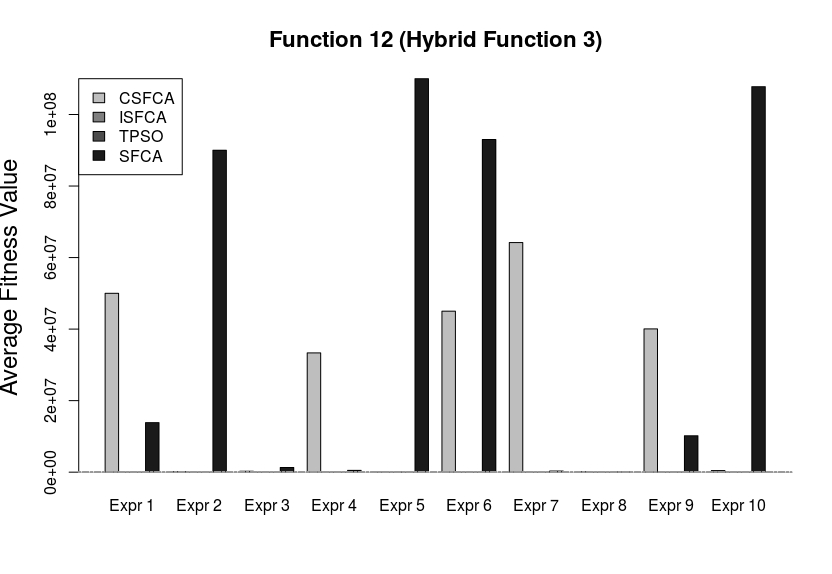
\includegraphics[scale=0.5]{func12_30}
	\centering
	\caption{Average fitness values for Function 12 with 30 dimensions}
	\label{func12_30}
\end{figure}

\section{Function 13: Composition Function 1}
This function is improved moderately in both 10- and 30-diemnsion cases. Table \ref{tbl13_10} and Figure \ref{func13_10} show that ISFCA and CSFCA improve the average fitness values for the 10-dimension case by 31\% and 10\% respectively. For the 30-dimension case, in Table \ref{tbl13_30} and \ref{func13_30}, we can see that ISFCA and CSFCA improve the performance by 51\% and 6\% respectively.
\begin{table}[h]
	\caption{function-13, dimension-10}
	\begin{tabular}{|c|c|c|c|c|}
		\hline
		& \textbf{SFPSO} & \textbf{CSFEP} & \textbf{SFEP} & \textbf{TPSO} \\ \hline
		\textbf{Median} & 1.626676E+03 & 1.750040E+03 & 2.101426E+03 & 1.623272E+03 \\ \hline
		\textbf{Mean} & 1.627982E+03 & 2.128914E+03 & 2.376883E+03 & 1.628781E+03 \\ \hline
		\textbf{Best} & 1.622335E+03 & 1.635087E+03 & 1.676418E+03 & 1.618919E+03 \\ \hline
		\textbf{StdDev} & 7.106025E+00 & 6.591729E+02 & 7.972695E+02 & 1.445686E+01 \\ \hline
	\end{tabular}
	\label{tbl13_10}
\end{table}

\begin{figure}[h]
	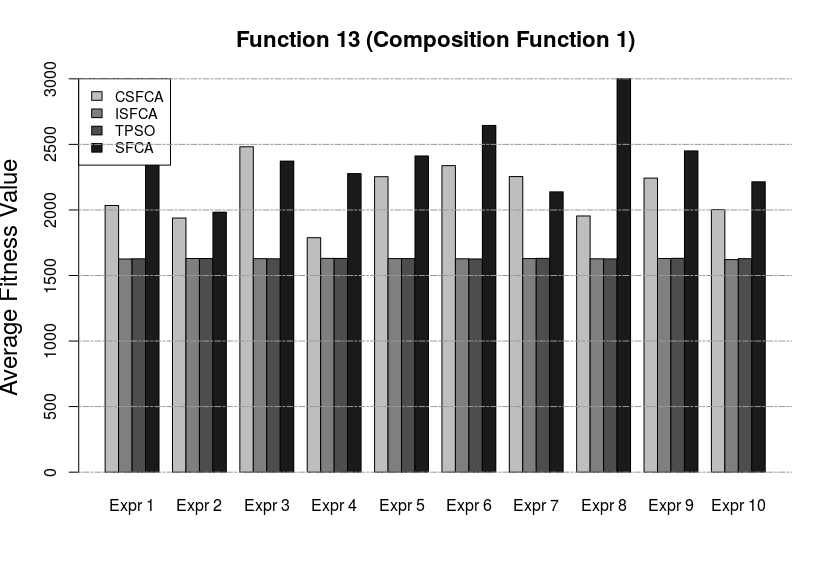
\includegraphics[scale=0.5]{func13_10}
	\centering
	\caption{Average fitness values for Function 13 with 10 dimensions}
	\label{func13_10}
\end{figure}

\begin{table}[h]
	\caption{function-13, dimension-30}
	\begin{tabular}{|c|c|c|c|c|}
		\hline
		& \textbf{SFPSO} & \textbf{CSFEP} & \textbf{SFEP} & \textbf{TPSO} \\ \hline
		\textbf{Median} & 1.727952E+03 & 2.442454E+03 & 3.419566E+03 & 1.742700E+03 \\ \hline
		\textbf{Mean} & 1.778258E+03 & 3.445463E+03 & 3.691270E+03 & 1.840829E+03 \\ \hline
		\textbf{Best} & 1.723534E+03 & 1.740536E+03 & 2.380543E+03 & 1.732389E+03 \\ \hline
		\textbf{StdDev} & 9.665278E+01 & 2.272010E+03 & 1.367277E+03 & 1.457157E+02 \\ \hline
	\end{tabular}
	\label{tbl13_30}
\end{table}
\begin{figure}[H]
	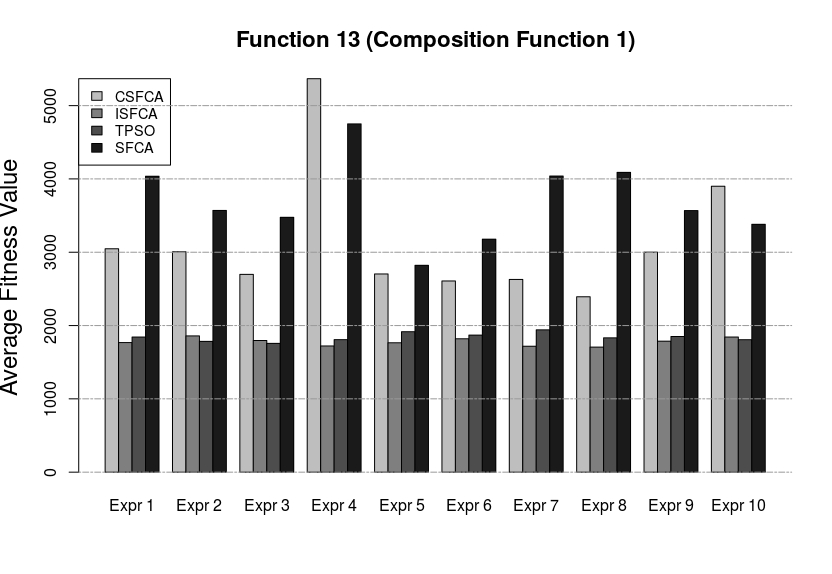
\includegraphics[scale=0.5]{func13_30}
	\centering
	\caption{Average fitness values for Function 13 with 30 dimensions}
	\label{func13_30}
\end{figure}

\section{Function 14: Composition Function 2}
For this function, the improvement made by our approaches is trivial about 1\% in the 10-dimension case. For the 30-dimension optimization, ISFCA and CSFCA improve the performance by 10\% and 4\% respectively.
\begin{table}[h]
	\caption{function-14, dimension-10}
	\begin{tabular}{|c|c|c|c|c|}
		\hline
		& \textbf{SFPSO} & \textbf{CSFEP} & \textbf{SFEP} & \textbf{TPSO} \\ \hline
		\textbf{Median} & 1.601795E+03 & 1.600173E+03 & 1.619095E+03 & 1.605406E+03 \\ \hline
		\textbf{Mean} & 1.602429E+03 & 1.607129E+03 & 1.623200E+03 & 1.606235E+03 \\ \hline
		\textbf{Best} & 1.601385E+03 & 1.591111E+03 & 1.597342E+03 & 1.604991E+03 \\ \hline
		\textbf{StdDev} & 1.577398E+00 & 1.953208E+01 & 2.617243E+01 & 1.478468E+00 \\ \hline
	\end{tabular}
	\label{tbl14_10}
\end{table}

\begin{figure}[h]
	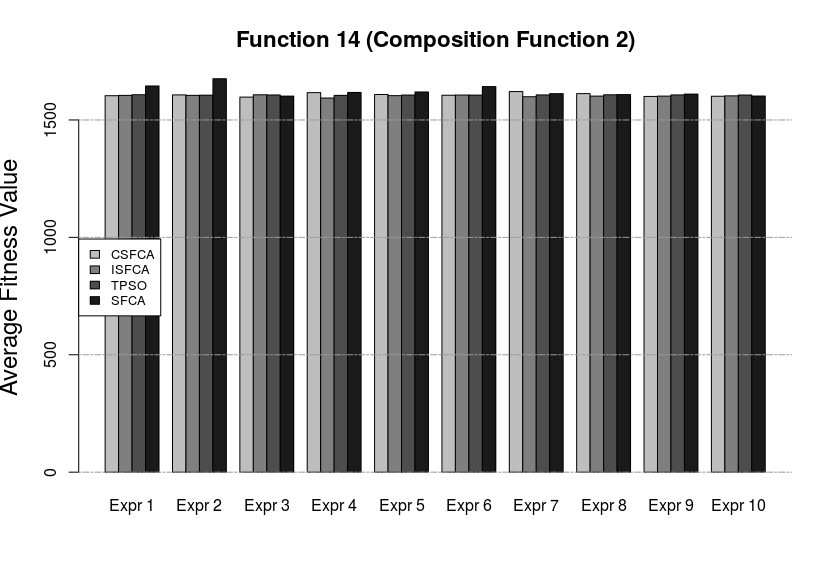
\includegraphics[scale=0.5]{func14_10}
	\centering
	\caption{Average fitness values for Function 14 with 10 dimensions}
	\label{func14_10}
\end{figure}

\begin{table}[h]
	\caption{function-14, dimension-30}
	\begin{tabular}{|c|c|c|c|c|}
		\hline
		& \textbf{SFPSO} & \textbf{CSFEP} & \textbf{SFEP} & \textbf{TPSO} \\ \hline
		\textbf{Median} & 1.675847E+03 & 1.731879E+03 & 1.820677E+03 & 1.664094E+03 \\ \hline
		\textbf{Mean} & 1.676279E+03 & 1.791878E+03 & 1.865010E+03 & 1.685711E+03 \\ \hline
		\textbf{Best} & 1.646723E+03 & 1.660532E+03 & 1.693461E+03 & 1.658174E+03 \\ \hline
		\textbf{StdDev} & 2.842502E+01 & 1.553106E+02 & 1.760265E+02 & 3.566090E+01 \\ \hline
	\end{tabular}
	\label{tbl14_30}
\end{table}
\begin{figure}[H]
	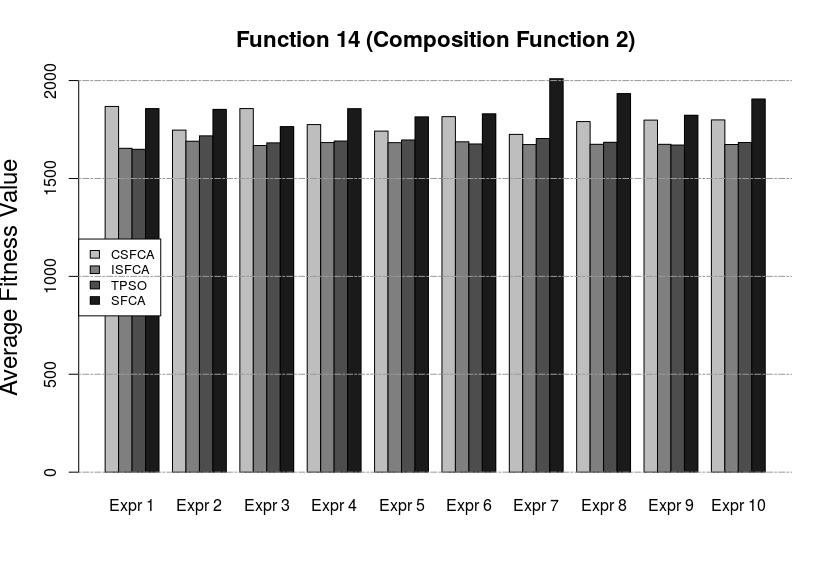
\includegraphics[scale=0.5]{func14_30}
	\centering
	\caption{Average fitness values for Function 14 with 30 dimensions}
	\label{func14_30}
\end{figure}

\section{Function 15: Composition Function 3}
For this function, ISFCA works better than CSFCA. ISFCA improves the average fitness value by 20\% and 29\% for 10- and 30-dimension cases respectively. On the other hand, CSFCA produces improvement only by 1\% and 16\% for 10- and 30-dimension cases respectively.
\begin{table}[h]
	\caption{function-15, dimension-10}
	\begin{tabular}{|c|c|c|c|c|}
		\hline
		& \textbf{SFPSO} & \textbf{CSFEP} & \textbf{SFEP} & \textbf{TPSO} \\ \hline
		\textbf{Median} & 1.560743E+03 & 1.913027E+03 & 1.949996E+03 & 1.853726E+03 \\ \hline
		\textbf{Mean} & 1.589476E+03 & 1.946018E+03 & 1.966892E+03 & 1.871080E+03 \\ \hline
		\textbf{Best} & 1.525130E+03 & 1.871689E+03 & 1.855628E+03 & 1.772940E+03 \\ \hline
		\textbf{StdDev} & 8.426385E+01 & 8.447839E+01 & 1.134500E+02 & 7.850262E+01 \\ \hline
	\end{tabular}
	\label{tbl15_10}
\end{table}

\begin{figure}[h]
	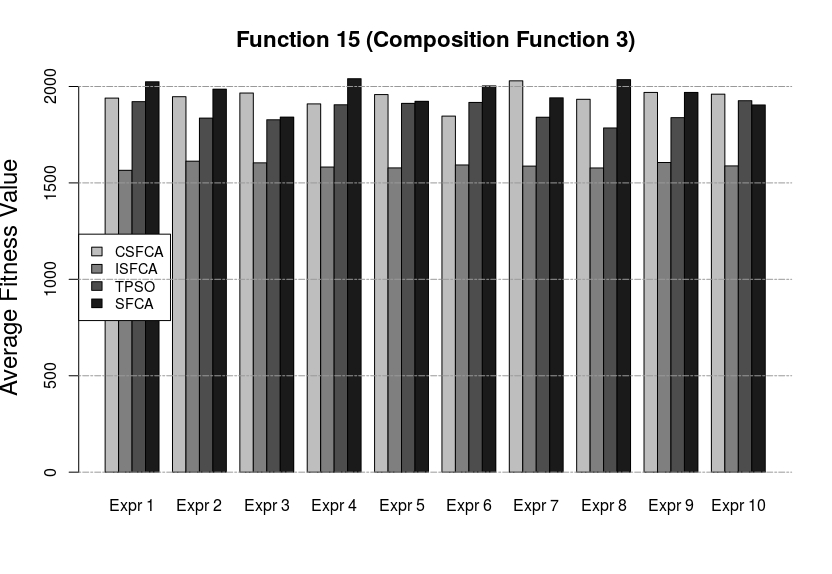
\includegraphics[scale=0.5]{func15_10}
	\centering
	\caption{Average fitness values for Function 15 with 10 dimensions}
	\label{func15_10}
\end{figure}

\begin{table}[h]
	\caption{function-15, dimension-30}
	\begin{tabular}{|c|c|c|c|c|}
		\hline
		& \textbf{SFPSO} & \textbf{CSFEP} & \textbf{SFEP} & \textbf{TPSO} \\ \hline
		\textbf{Median} & 2.565830E+03 & 2.760375E+03 & 3.096788E+03 & 2.511983E+03 \\ \hline
		\textbf{Mean} & 2.582142E+03 & 3.063021E+03 & 3.657078E+03 & 2.565208E+03 \\ \hline
		\textbf{Best} & 2.498940E+03 & 2.227419E+03 & 3.055342E+03 & 2.504910E+03 \\ \hline
		\textbf{StdDev} & 9.012990E+01 & 1.040607E+03 & 1.152769E+03 & 8.765290E+01 \\ \hline
	\end{tabular}
	\label{tbl15_30}
\end{table}
\begin{figure}[H]
	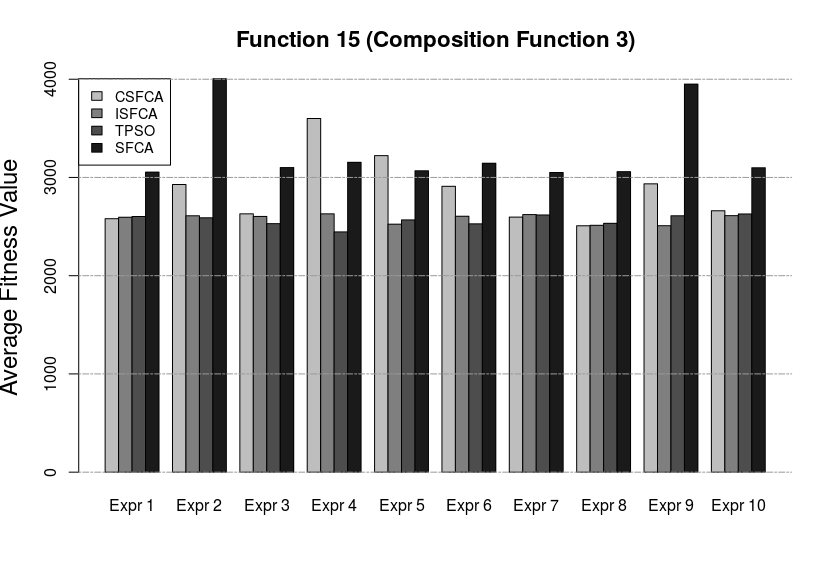
\includegraphics[scale=0.5]{func15_30}
	\centering
	\caption{Average fitness values for Function 15 with 30 dimensions}
	\label{func15_30}
\end{figure}
\section{Summary of Results}
In this chapter, we presented an extensive comparison of our proposed approaches with the standard social fabric algorithm \citet{ali2016leveraged} and Tribe-PSO \citet{chen2006tribe}. We chose these algorithms because both of them utilize multi-population and tribal strategies to improve the level of diversity in evolutionary algorithms. \newline
As we can in the tables and figures for the functions 1, 2, 8, 10, and 12, the new neighborhood restructuring strategy and the confidence-based normative ranges generated more tan 50\% improvement. It seems the proposed methods succeeded to help the individuals to avoid stagnation and local optima. \newline
For the functions 4, 7, 11, 13, 14, and 15 the new approaches improve the performance with a lower percentage between 10\% and 20\%. Although, for the remaining functions the generated improvement is trivial. We hypothesize that it occurred because of the high-level complexity of the benchmark functions we used. In the standard implementation of the IEEE-CEC2015 library, the functions are twisted and rotated to make it hard for optimization algorithms to get rid of local optima \citet{chen2014problem}. Also, as it is stated by above mentioned the No-Free Lunch Theorem,  it is not expected for an optimization algorithm to work well on all of the possible functions \citet{wolpert1997no}.
%For a Master's research this chapter represents the critical part where \textbf{you} are truly evaluated to determine whether you should be given your degree. Even more so for a PhD. Consider carefully what the University calendar states regarding the expectations for a master's thesis, paraphrased here.
%
%\begin{enumerate}
%\item {\textit{A Master�s thesis is an original lengthy essay.} The main implication here is that the essay is original, that is, it is completely newly written by you and does not contain any writings from others unless precisely quoted. Any paraphrased items must be cited.}
%\item {\textit{It must demonstrate that:}
%    \begin{itemize}
%    \item {students understand research methods;}
%    \item {students are capable to employ research methods;}
%    \item {students demonstrate command of the subject.}
%    \end{itemize}}
%\item {\textit{The work may be based on:}
%    \begin{itemize}
%    \item {original data;}
%    \item {original exercise from scholarly literature;}
%    \item {data by others.}
%    \end{itemize}}
%\item {\textit{The work must show that:}
%    \begin{itemize}
%    \item {appropriate research methods have been used;}
%    \item {appropriate methods of critical analysis supplied.}
%    \end{itemize}}
%\item {\textit{The work must contain:}
%    \begin{itemize}
%    \item {evidence of some new contribution;}
%    \item {evidence of a new perspective on existing knowledge.}
%    \end{itemize}}
%\end{enumerate}
%
%Only the last point uses the attribute \textit{new} and it refers almost entirely to giving a new perspective and analysis, even if based on data from others. This truly implies that this current chapter on evaluation and analysis of results is the most important and must be written with care. You are demonstrating here that, even if given data and methods from others, your skills of critical judgment and analysis are now at the level that you can give professional evaluations.
%
%Things are slightly different for a PhD. According to the Graduate Calendar: \\ 
%\textit{a doctoral dissertation must embody original work and constitute a significant contribution to knowledge in the candidate's field of study. It should contain evidence of broad knowledge of the relevant literature, and should demonstrate a critical understanding of the works of scholars closely related to the subject of the dissertation. Material embodied in the dissertation should, in the opinion of scholars in the field, merit publication.}
%
%\textit{The general form and style of dissertations may differ from department to department, but all dissertations shall be presented in a form which constitutes an integrated submission. The dissertation may include materials already published by the candidate, whether alone or in conjunction with others. Previously published materials must be integrated into the dissertation while at the same time distinguishing the student's own work from the work of other researchers. At the final oral examination, the doctoral candidate is responsible for the entire content of the dissertation. This includes those portions of co-authored papers which comprise part of the dissertation.}
%
%The second paragraph makes it clear that one must emphasize what is new and different from others, without arrogance, yet without being too subtle either. The first paragraph implies that for a PhD it is required that one approached an important open problem and gave a new solution altogether, making chapters 3, 4, 5 all part of the body of research being evaluated. In fact at times even the problem may be entirely new, thus including chapter 2 in the examination. This is in contrast to a Master's degree where the minimum requirement is for chapter 5 to be original.
%
%
%
%